\subsection{Worked example: removing one recommendation while preserving the others}
\label{sec:worked}

The example is one MovieLens pair from the stored $K=5$ sweep (exact method, $\alpha=0.5$, $\varepsilon=10^{-6}$, mask domain $D_u(t)$). It was chosen because setting C is recorded as optimal with a mask of size 1, the history has 12 movies, the mask domain has 12 interactions, and the cross-check status is confirmed. The target is a widely known title. It illustrates the procedure. It is not an estimate of average mask size or feasibility.

User 4739 is recommended, in order, 1.\ \emph{Godfather: Part II, The (1974)} (11.3328), 2.\ \emph{Shawshank Redemption, The (1994)} (11.0729), 3.\ \emph{Star Wars: Episode IV - A New Hope (1977)} (10.9434), 4.\ \emph{Star Wars: Episode VI - Return of the Jedi (1983)} (10.2361), 5.\ \emph{Pulp Fiction (1994)} (9.6114). The target is \emph{Star Wars: Episode VI - Return of the Jedi (1983)}, originally rank 4, score 10.2361. The three history movies that contribute most to its score are \emph{Star Wars: Episode V - The Empire Strikes Back (1980)} (2.6780), \emph{Star Wars: Episode I - The Phantom Menace (1999)} (1.3932), \emph{Sixth Sense, The (1999)} (0.8205).

The masked interaction is \emph{Star Wars: Episode V - The Empire Strikes Back (1980)}, which is among those three contributors. Its contribution is removed and the others stay.

Under C1+C2+C3 the solver returns $M$ of size 1: Star Wars: Episode V - The Empire Strikes Back (1980). The study configuration reports status optimal in 0.1137 seconds. The independent verifier accepts the mask under both $P$ and $P_\varepsilon$ (C1 = True, C2 = True, C3 = True). The stored $K=5$ record has status optimal, size 1, and the masks match. Enumeration of every subset of $D_u(t)$ (12 interactions) finds the same minimum size under $P$ (1) and under $P_\varepsilon$ (1). No smaller permitted mask satisfies C1+C2+C3 under either formulation.

After the mask the top five are 1.\ \emph{Godfather: Part II, The (1974)} (10.3997), 2.\ \emph{Shawshank Redemption, The (1994)} (10.1131), 3.\ \emph{Pulp Fiction (1994)} (8.6997), 4.\ \emph{Star Wars: Episode IV - A New Hope (1977)} (8.6464), 5.\ \emph{Schindler's List (1993)} (8.5450). \emph{Star Wars: Episode VI - Return of the Jedi (1983)} is not among them. The other four original movies remain. The replacement is \emph{Schindler's List (1993)} (rank 5, score 8.5450). Kendall's $\tau_a$ on the four retained movies, before against after, is 0.667.

\begin{table}[t]
\centering
\caption{Surviving evidence for the four movies that stay in the worked example. Each row is one original path whose contribution is at least $\tau_j$ and whose origin is not masked. Entity names are not in the rehashed Satori release, so the intermediate node is a relation and a rehashed id, or ``co-user''.}
\label{tab:worked}
\resizebox{\linewidth}{!}{%
\begin{tabular}{lcccccc}
\toprule
Retained movie & $\tau_j$ & relation & origin & via & $c(p)$ & survives \\
\midrule
Godfather: Part II, The (1974) & 0.086315 & actor & Godfather, The (1972) & rehashed-entity-2339 & 0.172631 & yes \\
Shawshank Redemption, The (1994) & 0.129473 & actor & Insider, The (1999) & rehashed-entity-3141 & 0.258946 & yes \\
Star Wars: Episode IV - A New Hope (1977) & 0.064737 & actor & Bridge on the River Kwai, The (1957) & rehashed-entity-2349 & 0.073985 & yes \\
Pulp Fiction (1994) & 0.016184 & actor & Sixth Sense, The (1999) & rehashed-entity-1401 & 0.032368 & yes \\
\bottomrule
\end{tabular}}
\end{table}

Masking Star Wars: Episode V - The Empire Strikes Back (1980) removes \emph{Star Wars: Episode VI - Return of the Jedi (1983)} from the top-five recommendations. The remaining four original movies stay in the list, and each retains at least one original evidence path meeting its contribution threshold. The edit is a change to the inputs of the scorer, followed by re-ranking. It is not a change to the interface, and this example is not evidence about privacy, conversion or trust.

On this pair the target-score heuristic that stops at removal masks Star Wars: Episode V - The Empire Strikes Back (1980). The verifier reports C1 = True, C2 = True, C3 = True. This particular removal happens to satisfy C2 and C3 as well, so it is not an example of collateral damage. The main-sample rate, not this pair, is the evidence that removal-only edits usually do not.

\begin{figure}[t]
\centering
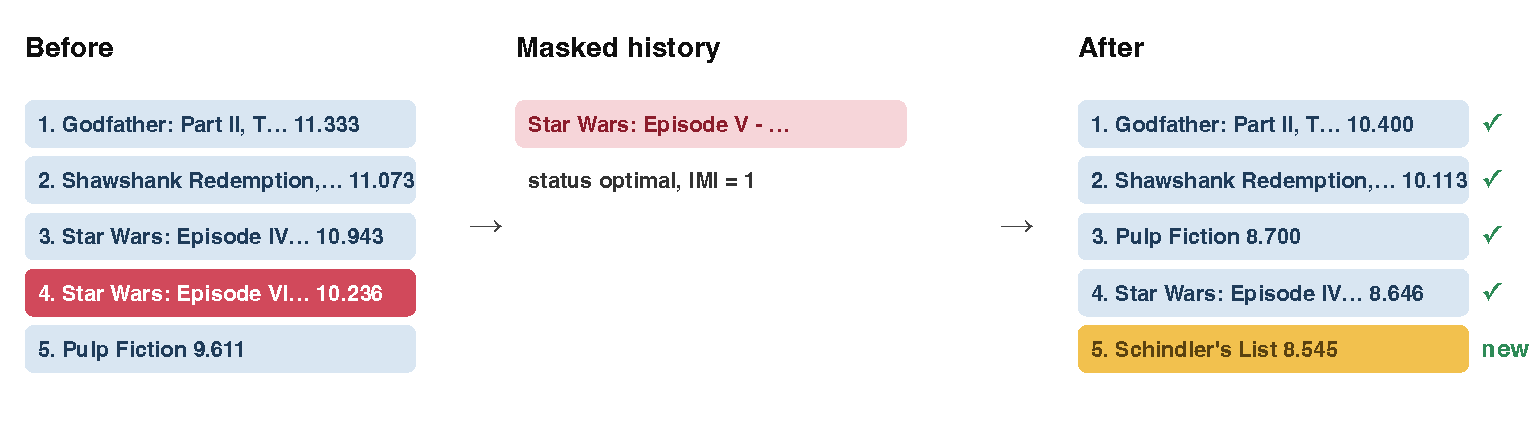
\includegraphics[width=\linewidth]{fig_worked.pdf}
\caption{Worked example, $K=5$. Left: the original list; the target is red. Centre: the masked history interaction. Right: the list after re-ranking. Blue rows are retained movies, the gold row is the replacement, and a tick marks a retained movie that keeps a qualifying path. Scores are the path-additive scores.}
\label{fig:worked}
\end{figure}

